\subsection{Multipliers}
\label{sec:implementation_multipliers}
\label{sec:implementation_multiplication}

While the simple arithmetic (addition, negation) of a point depends on its curve, algorithms for speeding up scalar
multiplication of points are often independent of the type of curve. For example, the Double-and-Add algorithm can
be applied to a point on any type of curve and result in exactly the same speed-up in computation time (compared to
naively adding a point continuously to an accumulator).

\begin{figure}[htb]
	\centering
	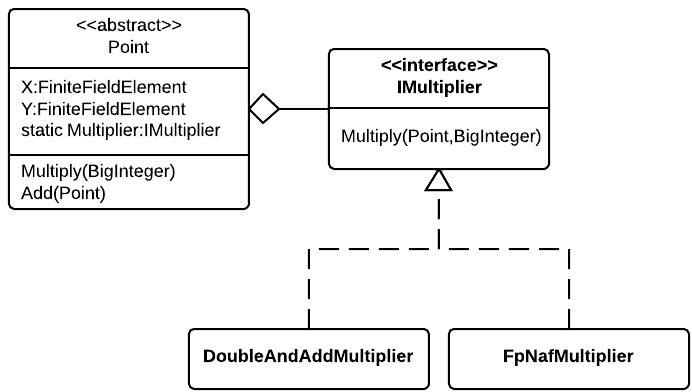
\includegraphics[width=0.7\textwidth]{implementation/multipliers}
	\caption{The relationship between points and multipliers. The multiplier is defined for all types of points (as it
		is set as a static property on the \texttt{Point} abstract class.}
\end{figure}

The possibility for changing a multiplier (and hence a multiplication algorithm) without having to change the code
performing the simple arithmetic both encourages such improvements, and enables performance comparisons of multiplication
algorithm candidates.

\textbf{Note: Some curves have tricks - like the montgomery ladder, which trades time for precomputed space. How can these
be implemented? Should the multiplier be set on a per-class basis instead of "for all points" once these are supported? Probably, yes.}

\textbf{Note: Point multiplication is covered in Hankerson pp. 95-?}
